\documentclass[UTF8,12pt]{article}
\usepackage{ctex}
\usepackage{indentfirst}
\usepackage{color}
\usepackage{hyperref}
\usepackage{graphicx}
\usepackage{subfigure}
\usepackage{pdfpages}
\usepackage{listings}
\hypersetup{
    hidelinks,
	colorlinks=true,
	allcolors=black,
	pdfstartview=Fit,
	breaklinks=true
}

\definecolor{dkgreen}{rgb}{0,0.6,0}
\definecolor{gray}{rgb}{0.5,0.5,0.5}
\definecolor{mauve}{rgb}{0.58,0,0.82}

\lstset{ %
  language=Octave,                % the language of the code
  basicstyle=\footnotesize,           % the size of the fonts that are used for the code
  numbers=left,                   % where to put the line-numbers
  numberstyle=\tiny\color{gray},  % the style that is used for the line-numbers
  stepnumber=2,                   % the step between two line-numbers. If it's 1, each line 
                                  % will be numbered
  numbersep=5pt,                  % how far the line-numbers are from the code
  backgroundcolor=\color{white},      % choose the background color. You must add \usepackage{color}
  showspaces=false,               % show spaces adding particular underscores
  showstringspaces=false,         % underline spaces within strings
  showtabs=false,                 % show tabs within strings adding particular underscores
  frame=single,                   % adds a frame around the code
  rulecolor=\color{black},        % if not set, the frame-color may be changed on line-breaks within not-black text (e.g. commens (green here))
  tabsize=2,                      % sets default tabsize to 2 spaces
  captionpos=b,                   % sets the caption-position to bottom
  breaklines=true,                % sets automatic line breaking
  breakatwhitespace=false,        % sets if automatic breaks should only happen at whitespace
  title=\lstname,                   % show the filename of files included with \lstinputlisting;
                                  % also try caption instead of title
  keywordstyle=\color{blue},          % keyword style
  commentstyle=\color{dkgreen},       % comment style
  stringstyle=\color{mauve},         % string literal style
  escapeinside={\%*}{*)},            % if you want to add LaTeX within your code
  morekeywords={*,...}               % if you want to add more keywords to the set
}


\setlength{\parindent}{2em}

\begin{document}



\begin{center}
    \tableofcontents
\end{center}
\newpage

\section{实验名称}
进程管理与内存分配模拟程序

\section{实验目的}
\begin{enumerate}
    \item 设计编写OS进程与内存管理模拟程序,模拟OS进程的创建、阻塞、唤醒、撤销等进程控制以及OS内存管理方法和过程,加深操作系统进程控制原语主要任务和过程的理解,加深操作系统内存分配的基本策略,加深操作系统以进程为核心的完整架构的理解
    \item 提高综合性实验的分析、设计及编程实现能力
\end{enumerate}

\section{实验内容}
设计一个OS进程与内存管理模拟程序,要求:
(1)程序运行后提供一个交互界面或窗口,允许用户输入以下命令并可以对命令进行解释执行(即执行OS的创建进程原语)
\begin{itemize}
    \item creatproc:提交作业命令,要求用户提供作业估计运行时长和内存大小需求。该命令的解释执行过程为对该作业创建对应的进程,完成PCB建立、存储空间分配等工作
    \item killproc 进程号:终止进程命令。该命令的解释执行过程为对进程进行撤销,回收存储空间和PCB
    \item iostartproc 进程号:阻塞进程命令。该命令的解释执行过程为对处于运行状态的进程进行阻塞操作,进程状态转为阻塞状态
    \item iofinishproc 进程号:阻塞进程命令。该命令的解释执行过程为对处于阻塞状态的进程进行唤醒操作,进程状态转为就绪状态
    \item psproc:显示所有进程状态命令。该命令的解释执行过程为显示出所有进程的状态信息,主要包括进程id,进程状态,存储空间地址
    \item mem:显示内存空间使用情况信息。该命令的解释执行过程为显示内存空间的占用和空闲情况
\end{itemize}

(2)设计思路提示:内存空间可用数组模拟,主要原语模拟实现,包括创建进程,终止进程,阻塞进程,唤醒进程,进程调度等原语。进程调度算法可选择 FCFS、RR、SJF中任意一种。内存分配可选择可变分区策略或页式内存分配方案中任意一种。

(3)程序设计语言不限

\section{准备知识}
\subsection{进程控制块(PCB)}
进程控制块PCB包含了有关进程的描述信息、控制信息以及资源信息,是进程动态特征的集中反映。系统根据PCB感知进程的存在和通过PCB中所包含的各项变量的变化,掌握进程所处的状态以达到控制进程活动的目的

\subsection{进程的基本状态}
包括创建、撤销、阻塞、唤醒、就绪、运行、完成等状态

\subsection{进程控制主要原语}
进程创建原语create;

进程撤销原语kill;

进程阻塞原语block;

进程唤醒原语wakeup;

进程调度原语schedule

\subsection{进程调度算法}
FCFS、SJF、RR、高响应比优先、优先级调度等

\subsection{内存分配策略及对应的数据结构}
内存分配策略包括固定分区分配、可变分区分配、页式内存分配、段式内存分配、段页式内存分配等

\section{实验设计}
\subsection{程序设计语言}
编程语言:java 17.0.4.1

编译器:IDEA

\subsection{进程调度和内存分配策略选择}
本次实验中,进程调度策略采用了FCFS(先来先服务)策略,内存分配策略采用了可变分区分配策略
\subsubsection{FCFS策略}
FCFS(先来先服务)策略是一种非抢占式的调度策略,即一旦CPU分配给某进程,那么该进程将一直占用CPU直到完成或者发生某种事件而被迫放弃CPU。FCFS策略的优点是简单易于实现,但是其缺点也很明显,即平均等待时间较长,不利于提高CPU的利用率。


\subsubsection{可变分区分配策略}
可变分区分配策略是指内存空间被分为若干个不相等的分区,每个分区可装入一个作业,作业装入内存时,根据作业的大小,为其分配一个合适的分区,若无合适的分区,则将其放入外存的后备队列中,等待空闲分区出现。当作业完成后,释放其所占用的分区,使之成为空闲分区,以便接纳新的作业。

\subsection{数据结构设计}
\subsubsection{进程控制块PCB}
进程控制块PCB包含了有关进程的描述信息、控制信息以及资源信息,是进程动态特征的集中反映。系统根据PCB感知进程的存在和通过PCB中所包含的各项变量的变化,掌握进程所处的状态以达到控制进程活动的目的。

在本实验中,封装了PCB类,包含了进程的id、状态、进程运行时间、内存大小、内存起始地址等信息,同时提供了对应的get和set方法,重写了tostring方法,将PCB中存储的各类属性以一定的顺序返回,方便后续的输出;同时提供了stateToString方法,将状态码转换为状态,方便输出。

PCB类的定义如下:
\begin{lstlisting}[title=PCB类定义,frame=shadowbox]
    public class PCB {//进程控制块
    private int pid;//进程标识符
    private String state;//进程状态
    private long time;//进程运行时间
    private int size;//进程所需内存大小
    private int priority;//进程优先级
    private boolean mark;//进程是否被标记
    private int memoryAddress;//进程内存地址
    private boolean Sched;//进程是否被调度

    //构造函数
    public PCB(){
        mark = false;
    }
    
    public int getPid() {
        return pid;
    }

    public void setPid(int pid) {
        this.pid = pid;
    }

    public String getState() {
        return state;
    }

    public void setState(String state) {
        this.state = state;
    }

    public int getPriority() {
        return priority;
    }

    public void setPriority(int priority) {
        this.priority = priority;
    }

    public boolean getMark() {
        return mark;
    }

    public void setMark(boolean mark) {
        this.mark = mark;
    }

    public int getMemoryAddress() {
        return memoryAddress;
    }

    public void setMemoryAddress(int memoryAddress) {
        this.memoryAddress = memoryAddress;
    }

    public boolean isSched() {
        return Sched;
    }

    public void setSched(boolean sched) {
        Sched = sched;
    }

    public long getTime() {
        return time;
    }

    public void setTime(long time) {
        this.time = time;
    }

    public int getSize() {
        return size;
    }

    public void setSize(int size) {
        this.size = size;
    }

    @Override
    public String toString() {
        return "{" +
                "pid=" + pid +
                ", state='" + stateToString(state) + '\'' +
                ", memoryAddress=" + memoryAddress +
                ", time=" + time/1000 +
                '}'+'\n';
    }

    private String stateToString(String state){//将状态码转换为状态
        switch(state){
            case "3" : return "Ready";
            case "4" : return "Block";
            case "5" : return "Run";
            default:return "Unknow";
        }
    }
}
\end{lstlisting}

\subsubsection{自由内存分区表}
自由内存分区表是指内存中空闲分区的集合,每个空闲分区由起始地址和长度组成。在本实验中,封装了FreeBlock类,包含了空闲分区的编号和长度,同时提供了对应的get和set方法,重写了tostring方法,将FreeBlock中存储的各类属性以一定的顺序返回,方便后续的输出。

FreeBlock类的定义如下:
\begin{lstlisting}[title=FreeBlock类定义,frame=shadowbox]
public class FreeBlock {//空闲块
    int index;
    int length;

    public FreeBlock(int index, int length) {
        this.index = index;
        this.length = length;
    }

    public int getIndex() {
        return index;
    }

    public void setIndex(int index) {
        this.index = index;
    }

    public int getLength() {
        return length;
    }

    public void setLength(int length) {
        this.length = length;
    }

    @Override
    public String toString() {
        return "FreeBlock{" +
                "index=" + index +
                ", length=" + length +
                '}';
    }
}
\end{lstlisting}

\subsubsection{状态码接口}
为了方便后续的状态码转换,封装了States接口,其中包含了进程的各种状态码,方便后续的调用。

状态码接口的定义如下:
\begin{lstlisting}[title=状态码接口定义,frame=shadowbox]
public interface States {
    String PROCESS_CREATE = "1";//创建
    String PROCESS_REVOKE = "2";//撤销
    String PROCESS_READY = "3";//就绪
    String PROCESS_BLOCK = "4";//阻塞
    String PROCESS_RUN = "5";//运行
}
\end{lstlisting}

其中,状态码为1表示创建,2表示撤销,3表示就绪,4表示阻塞,5表示运行。

\subsection{主要类设计}
\subsubsection{内存管理类}
内存管理类ManageMemory主要用于控制内存的分配和回收,其中包含了模拟总内存大小(本实验中设置100,从0号单元开始计数)、空闲内存列表等成员变量,主要实现函数是分配内存和回收内存。

分配内存函数allocMemory的定义如下:
\begin{lstlisting}[title=分配内存函数定义,frame=shadowbox]
    public static boolean allocateMemory(PCB pcb) {//分配内存,可变分区,最佳适应算法
        //对升序排序,挑选最合适空闲块
        freeBlocksList.sort((o1, o2) -> {
            if (o1.getLength() < o2.getLength()) return -1;
            return 1;
        });

        boolean flag = false;
        for (int i = 0; i < freeBlocksList.size(); i++) {
            FreeBlock a = freeBlocksList.get(i);
            if (a.getLength() < pcb.getSize()) continue;
            pcb.setMemoryAddress(a.getIndex());
            if (a.getLength() == pcb.getSize()) {
                freeBlocksList.remove(a);
                flag = true;
                break;
            }
            a.setIndex(a.getIndex() + pcb.getSize());
            a.setLength(a.getLength() - pcb.getSize());
            flag = true;
            break;
        }
        return flag;
    }
\end{lstlisting}

其中,首先对空闲内存列表进行升序排序,然后遍历空闲内存列表,找到第一个满足条件的空闲内存块,将进程的内存地址设置为该空闲内存块的起始地址:
\begin{itemize}
    \item 如果该空闲内存块的大小正好等于进程的内存大小,则将该空闲内存块从空闲内存列表中删除
    \item 否则将该空闲内存块的起始地址设置为该空闲内存块的起始地址加上进程的内存大小,将该空闲内存块的大小设置为该空闲内存块的大小减去进程的内存大小
\end{itemize}

回收内存函数retrieveMemory的定义如下:
\begin{lstlisting}[title=回收内存函数定义,frame=shadowbox]
    public static void retrieveMemory(PCB pcb) {//释放内存
        freeBlocksList.sort((o1, o2) -> {
            if (o1.getIndex() < o2.getIndex()) return -1;
            return 1;
        });
        //回收内存

        if (freeBlocksList.size() == 0) {
            freeBlocksList.add(new FreeBlock(pcb.getMemoryAddress(), pcb.getSize()));
            return;
        }

        int i = 0;
        FreeBlock a;
        for (; i < freeBlocksList.size(); i++) {
            a = freeBlocksList.get(i);
            if (a.getIndex() > pcb.getMemoryAddress()) break;
        }

        System.out.println("第" + i + "个空闲块");
        if (i == 0) {
            FreeBlock back = freeBlocksList.get(i);
            if (back.getIndex() == pcb.getMemoryAddress() + pcb.getSize()) {
                back.setIndex(pcb.getMemoryAddress());
                back.setLength(pcb.getSize() + back.getLength());
            } else {
                freeBlocksList.add(new FreeBlock(pcb.getMemoryAddress(), pcb.getSize()));
            }
            return;
        }

        if (i >= freeBlocksList.size()) {
            FreeBlock front = freeBlocksList.get(i - 1);
            if (front.getIndex() + front.getLength() == pcb.getMemoryAddress()) {
                front.setLength(front.getLength() + pcb.getSize());
            } else {
                freeBlocksList.add(new FreeBlock(pcb.getMemoryAddress(), pcb.getSize()));
            }
            return;
        }

        FreeBlock front = freeBlocksList.get(i - 1);
        FreeBlock back = freeBlocksList.get(i);
        if (front.getIndex() + front.getLength() == pcb.getMemoryAddress() && back.getIndex() == pcb.getMemoryAddress() + pcb.getSize()) {
            front.setLength(front.getLength() + back.getLength() + pcb.getSize());
            freeBlocksList.remove(back);
        } else if (front.getIndex() + front.getLength() == pcb.getMemoryAddress()) {
            front.setLength(front.getLength() + pcb.getSize());
        } else if (back.getIndex() == pcb.getMemoryAddress() + pcb.getSize()) {
            back.setIndex(pcb.getMemoryAddress());
            back.setLength(pcb.getSize() + back.getLength());
        } else {
            freeBlocksList.add(new FreeBlock(pcb.getMemoryAddress(), pcb.getSize()));
        }
    }
\end{lstlisting}

其中,首先将空闲内存块升序排序,然后将当前释放的内存块插入到空闲内存列表中,然后遍历空闲内存列表,将相邻的空闲内存块合并。

\subsubsection{PCB管理类}
PCB管理类ManagePCB主要用于PCB各属性的分配和回收,其中包含了PCB数组(PCB数量为10)、PCB的id等变量,主要用于模拟PCB的分配和回收。

PCB管理类ManagePCB的定义如下:
\begin{lstlisting}[title=PCB管理类定义,frame=shadowbox]
public class ManagePCB {
    private static int PID = 0;
    private static PCB[] pcbs = new PCB[]{new PCB(),new PCB(),new PCB(),new PCB(),new PCB(),new PCB(),new PCB(),new PCB(),new PCB(),new PCB()};


    public static PCB getFreePCB(){//获取空闲PCB
        for(PCB a:pcbs){
            if(a.getMark() == false)return a;
        }
        return null;
    }

    public static PCB getPCB(int pid){
        for(PCB a:pcbs){
            if(a.getPid() == pid)return a;
        }
        return null;
    }

    public static void retrievePCB(PCB pcb){
        pcb.setMark(false);
    }
    public static int getPID(){
        return PID++;
    }


}
\end{lstlisting}

其中,getFreePCB函数用于获取空闲的PCB,getPCB函数用于根据进程的id获取对应的PCB,retrievePCB函数用于回收PCB,getPID函数用于获取新的进程id。在设计中,PCB是否被占用很巧妙地转化成了PCB是否被标记,这样可以很方便地进行PCB的分配和回收,同时避免了脏数据的产生。

\subsubsection{进程管理类}
进程管理类ManageProcess包含了进程列表、就绪队列、阻塞队列、运行队列等变量,主要用于存储进程的信息,将进程调度的工作进行切割,单独成类,方便后续的调用。由于存放了三个队列一个列表,因此需要提供对应的插入列表或者队列的函数。

进程管理类ManageProcess的定义如下:
\begin{lstlisting}[title=进程管理类定义,frame=shadowbox]
    public class ManageProcess {//进程队列
    //四个static数组保存数据
    private static List<Process> processes = Collections.synchronizedList(new ArrayList<>());//进程列表
    private static Queue<Process> ReadyList = new LinkedList<>();//就绪队列
    private static Queue<Process> RunList = new LinkedList<>();//运行队列
    private static Queue<Process> BlockList = new LinkedList<>();//阻塞队列

    //两个插入函数,往static数组插入内容
    public static void insert(Queue<Process> List,Process process){
        List.offer(process);
    }

    public static void insert(List<Process> List,Process process){
        List.add(process);
    }


    public static Process getProcess(PCB pcb){
        for(Process a:processes){
            if(a.getPcb() == pcb)return a;
        }
        return null;
    }
    public static Queue<Process> getReadyList() {
        return ReadyList;
    }

    public static Queue<Process> getRunList() {
        return RunList;
    }
    public static boolean isFull(){//cpu最多同时处理三个进程
        if(RunList.size() == 3)return true;
        return false;
    }

    public static Queue<Process> getBlockList() {
        return BlockList;
    }

    public static List<Process> getProcesses() {
        return processes;
    }

}
\end{lstlisting}

其中,insert函数用于插入进程到对应的列表或者队列中,getProcess函数用于根据进程的PCB获取对应的进程,getReadyList函数用于获取就绪队列,getRunList函数用于获取运行队列,isFull函数用于判断运行队列是否已满(最多同时处理3个进程),getBlockList函数用于获取阻塞队列,getProcesses函数用于获取进程列表。

\subsubsection{进程调度类}
本类是整个程序中最为重要的类,主要用于模拟进程的调度,包含了FCFS调度算法的实现,同时包含了进程的创建、撤销、阻塞、唤醒等函数,是整个程序的核心。

在创建进程时,首先获取一个空闲的PCB,然后根据用户输入的进程运行时间和内存大小,设置PCB的各项属性,然后将PCB插入到进程列表中,然后调用内存分配函数,分配内存,最后将进程插入到就绪队列中。

在撤销进程时,首先根据用户输入的进程id获取对应的PCB,然后根据PCB获取对应的进程,然后调用内存回收函数,回收内存,最后将进程从进程列表中删除。

在阻塞进程时,首先根据用户输入的进程id获取对应的PCB,然后根据PCB获取对应的进程,然后将进程从相应队列中删除,最后将进程插入到阻塞队列中,更新进程还需要运行的时间。

在唤醒进程时,首先根据用户输入的进程id获取对应的PCB,然后根据PCB获取对应的进程,然后将进程从阻塞队列中删除,最后将进程插入到就绪队列中。

在进程调度时,首先判断运行队列是否已满,如果已满,则直接返回,否则从就绪队列中获取一个进程,然后将进程插入到运行队列中,更新进程的状态,最后将进程的状态设置为运行。

进程调度类的定义如下:
\begin{lstlisting}[title=进程调度类定义,frame=shadowbox]
    public class Process {//进程控制
    private PCB pcb;

    private Timer t;
    private ProcessStop task;
    private long startTime;
    private long pauseTime;
    private Date date = new Date();

    public Process(PCB pcb) {
        this.pcb = pcb;
        creat();
    }

    public void creat(){//创建进程
        pcb.setMark(true);
        pcb.setPid(ManagePCB.getPID());
        if(ManageMemory.allocateMemory(pcb)){//分配内存
            pcb.setState(States.PROCESS_READY);
            ManageProcess.insert(ManageProcess.getProcesses(),this);
            ManageProcess.insert(ManageProcess.getReadyList(),this);
        }
        else{
            pcb.setState(States.PROCESS_BLOCK);
            ManageProcess.insert(ManageProcess.getProcesses(),this);
            ManageProcess.insert(ManageProcess.getBlockList(),this);
        }
    }

    public void kill(){//撤销进程
        pcb.setSched(false);
        if(pcb.getState().equals(States.PROCESS_RUN)){//运行状态撤销
            pcb.setSched(true);
            ManageProcess.getRunList().remove(ManageProcess.getProcess(pcb));
            ManageMemory.retrieveMemory(this.pcb);
        }
        if(pcb.getState().equals(States.PROCESS_READY)){//就绪状态撤销
            ManageProcess.getReadyList().remove(ManageProcess.getProcess(pcb));
            ManageMemory.retrieveMemory(this.pcb);
        }
        if(pcb.getState().equals(States.PROCESS_BLOCK)){//阻塞状态撤销
            ManageProcess.getBlockList().remove(ManageProcess.getProcess(pcb));
            ManageMemory.retrieveMemory(this.pcb);
        }
        ManagePCB.retrievePCB(this.pcb);
        ManageProcess.getProcesses().remove(this);
    }

    public void block(){//阻塞进程
        //Timer Stop
        date.setTime(System.currentTimeMillis());
        pauseTime = date.getTime();
        pcb.setTime(pcb.getTime() - (pauseTime - startTime));
        t.cancel();
        task.cancel();
        //退出RunList
        ManageProcess.getRunList().remove(this);
        //——>BlockList
        ManageProcess.insert(getBlockList(),this);
        //State->Block
        pcb.setState(States.PROCESS_BLOCK);
    }

    public void wakeup(){//唤醒进程
        ManageProcess.getBlockList().remove(this);
        pcb.setState(States.PROCESS_READY);
        ManageProcess.insert(ManageProcess.getReadyList(),this);
    }

    public void schedule(){//时间分配
        t = new Timer();
        task = new ProcessStop(this);
        date.setTime(System.currentTimeMillis());
        startTime = date.getTime();
        t.schedule(task,pcb.getTime());
    }

    public PCB getPcb() {
        return pcb;
    }

    public Timer getT() {
        return t;
    }

    public ProcessStop getTask() {
        return task;
    }

    public void setT(Timer t) {
        this.t = t;
    }

    public void setTask(ProcessStop task) {
        this.task = task;
    }

    public long getStartTime() {
        return startTime;
    }

    public void setStartTime(long startTime) {
        this.startTime = startTime;
    }

    public long getPauseTime() {
        return pauseTime;
    }

    public void setPauseTime(long pauseTime) {
        this.pauseTime = pauseTime;
    }

    @Override
    public String toString() {
        return pcb.toString();
    }
}
\end{lstlisting}

其中,ProcessStop类用于模拟运行进程的停止,ProcessStop类的定义如下:

\begin{lstlisting}[title=ProcessStop类定义,frame=shadowbox]
    class ProcessStop extends TimerTask {
        private Process process;
    
        public ProcessStop(Process process) {
            this.process = process;
        }
    
        @Override
        public void run() {
            process.kill();
        }
    
    }
\end{lstlisting}

\subsubsection{控制台类}
控制台类Console主要用于模拟控制台,包含了主函数和控制台的各种命令,主要用于模拟用户的输入,方便后续的调用。

在控制台界面的设计中,使用了Java swing编写了一个简单的控制台界面,方便用户的输入和输出,同时使用了JTextArea组件,方便用户的输出。

窗体实现的代码如下:
\begin{lstlisting}[title=窗体实现代码,frame=shadowbox]
    public static void main(String[] args) {
        JFrame frame = new JFrame("进程管理与内存分配模拟程序");
        outputTextArea.setFont(new Font("宋体", Font.BOLD, 20));
        outputTextArea.setEditable(false);
        outputTextArea.setBackground(Color.cyan);

        inputTextField.setBackground(Color.lightGray);
        JScrollPane scrollPane = new JScrollPane(outputTextArea);
        scrollPane.setVerticalScrollBarPolicy(JScrollPane.VERTICAL_SCROLLBAR_ALWAYS);

        frame.getContentPane().setLayout(new BorderLayout());
        frame.getContentPane().add(scrollPane, BorderLayout.CENTER);
        frame.getContentPane().add(inputTextField, BorderLayout.SOUTH);

        outputTextArea.append("--------------进程管理与内存分配模拟程序--------------\n");
        outputTextArea.append("--------------createproc 时间 内存大小:提交作业命令---\n--------------killproc 进程号:终止进程---------------\n--------------iostartproc 进程号:阻塞进程命令--------\n--------------iofinishproc 进程号:阻塞进程唤醒命令----\n--------------psproc:显示所有进程状态命令------------\n--------------mem:显示内存空间使用情况信息------------\n\n");

        inputTextField.addActionListener(new ActionListener() {
            @Override
            public void actionPerformed(ActionEvent e) {
                String content = inputTextField.getText();
                inputTextField.setText("");
                process(content);
            }
        });

        frame.setDefaultCloseOperation(JFrame.EXIT_ON_CLOSE);
        frame.setBounds(500, 200, 800, 600);
        frame.setVisible(true);
        new Scheduler().start();
    }
\end{lstlisting}

在控制台类中,主要实现了process函数,用于解析用户的输入,也就是说输入相应的原语后,对消息进行分割,对原语进行匹配解析,然后调用相应的函数,方便后续的调用。

键入了createproc命令,则对命令进行切割,分别解析出进程运行时间和内存大小,然后调用创建进程函数,创建进程。

\begin{lstlisting}[title=键入createproc,frame=shadowbox]
    if (command.startsWith("createproc ")) {
            // 得到进程估计运行时间和所需内存大小
            String[] contents = command.split(" ");
            // 获取空闲PCB
            PCB pcb = ManagePCB.getFreePCB();
            // 失败的情况
            if (pcb == null) {
                outputTextArea.append("创建进程失败,没有空闲的PCB" + "\n");
                return;
            }
            // 成功就创建新进程
            pcb.setTime(Integer.parseInt(contents[1]) * 1000);
            pcb.setSize(Integer.parseInt(contents[2]));
            new Process(pcb);
            outputTextArea.append(ManageProcess.getProcesses().toString() + "\n");
        }
\end{lstlisting}

键入了killproc命令,则对命令进行切割,分别解析出进程id,然后调用撤销进程函数,撤销进程。

\begin{lstlisting}[title=键入killproc,frame=shadowbox]
    else if (command.startsWith("killproc ")) {
        String[] contents = command.split(" ");
        PCB pcb = ManagePCB.getPCB(Integer.parseInt(contents[1]));
        if (pcb == null) {
            outputTextArea.append("该进程不存在" + "\n");
            return;
        }
        ManageProcess.getProcess(pcb).kill();
        outputTextArea.append(ManageProcess.getProcesses().toString() + "\n");
    }
\end{lstlisting}

键入了iostartproc命令,则对命令进行切割,分别解析出进程id,然后调用阻塞进程函数,阻塞进程。

\begin{lstlisting}[title=键入iostartproc,frame=shadowbox]
    else if (command.startsWith("iostartproc ")) {
        String[] contents = command.split(" ");
        PCB pcb = ManagePCB.getPCB(Integer.parseInt(contents[1]));
        if (pcb == null) {
            outputTextArea.append("该进程不存在" + "\n");
            return;
        }
        // 判断是否被调度
        if (ManageProcess.getProcess(pcb) == null) {
            outputTextArea.append("该进程未被调度,阻塞操作失败" + "\n");
            return;
        }
        ManageProcess.getProcess(pcb).block();
        outputTextArea.append(ManageProcess.getProcesses().toString() + "\n");
    }
\end{lstlisting}

键入了iofinishproc命令,则对命令进行切割,分别解析出进程id,然后调用唤醒进程函数,唤醒进程。

\begin{lstlisting}[title=键入iofinishproc,frame=shadowbox]
    else if (command.startsWith("iofinishproc ")) {
        String[] contents = command.split(" ");
        PCB pcb = ManagePCB.getPCB(Integer.parseInt(contents[1]));
        if (pcb == null) {
            outputTextArea.append("该进程不存在" + "\n");
            return;
        }
        ManageProcess.getProcess(pcb).wakeup();
        outputTextArea.append(ManageProcess.getProcesses().toString() + "\n");
    }
\end{lstlisting}

键入了psproc命令,则调用显示进程状态函数,显示进程状态。

\begin{lstlisting}[title=键入psproc,frame=shadowbox]
    else if (command.equals("psproc")) {
        outputTextArea.append(ManageProcess.getProcesses().toString() + "\n");
    }
\end{lstlisting}

键入了mem命令,则调用显示内存状态函数,显示内存状态。

\begin{lstlisting}[title=键入mem,frame=shadowbox]
    else if (command.equals("mem")) {
        ManageMemory.getFreeBlocksList().sort((o1, o2) -> {
            if (o1.getIndex() < o2.getIndex()) return -1;
            return 1;
        });

        ManageProcess.getProcesses().sort((o1, o2) -> {
            if (o1.getPcb().getMemoryAddress() < o2.getPcb().getMemoryAddress()) return -1;
            return 1;
        });

        int i = 0, j = 0, k = ManageProcess.getProcesses().size(), t = ManageMemory.getFreeBlocksList().size();
        List<Process> processes = ManageProcess.getProcesses();
        List<FreeBlock> freeBlocksList = ManageMemory.getFreeBlocksList();
        while (i < k && j < t) {
            if (processes.get(i).getPcb().getMemoryAddress() < freeBlocksList.get(j).getIndex()) {
                outputTextArea.append(processes.get(i).getPcb().getMemoryAddress() + " --- " + (processes.get(i).getPcb().getMemoryAddress() + processes.get(i).getPcb().getSize() - 1) + "  分配给" + processes.get(i).getPcb().getPid() + "号进程" + "\n");
                i++;
            } else {
                outputTextArea.append(freeBlocksList.get(j).getIndex() + " --- " + (freeBlocksList.get(j).getIndex() + freeBlocksList.get(j).getLength() - 1) + "空闲" + "\n");
                j++;
            }
        }
        if (i < k) {
            while (i < k) {
                outputTextArea.append(processes.get(i).getPcb().getMemoryAddress() + " --- " + (processes.get(i).getPcb().getMemoryAddress() + processes.get(i).getPcb().getSize() - 1) + "  分配给" + processes.get(i).getPcb().getPid() + "号进程" + "\n");
                i++;
            }
        }
        if (j < t) {
            while (j < t) {
                outputTextArea.append(freeBlocksList.get(j).getIndex() + " --- " + (freeBlocksList.get(j).getIndex() + freeBlocksList.get(j).getLength() - 1) + "  空闲" + "\n");
                j++;
            }
        }
    }
\end{lstlisting}


\section{运行结果}
\subsection{初始运行界面}
\begin{figure}[htbp]
    \centering
    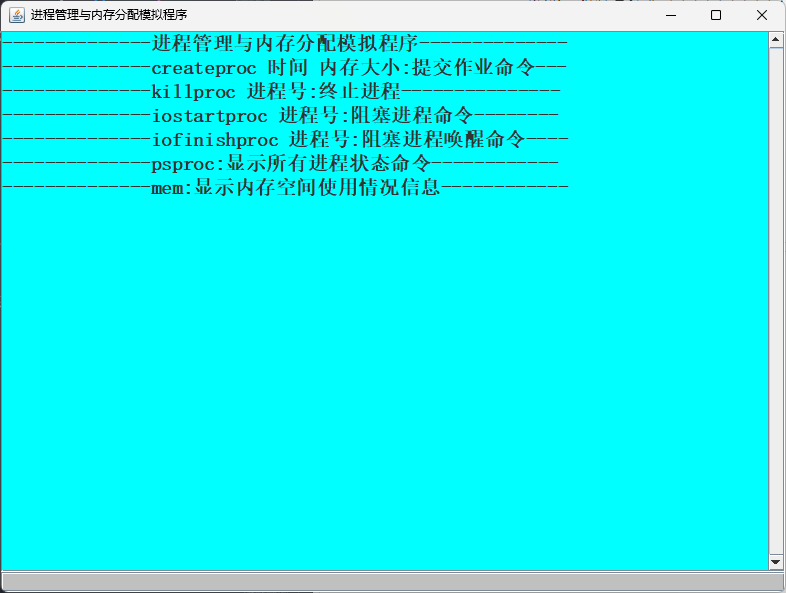
\includegraphics[width=0.5\textwidth]{img/1.png}
    \caption{初始运行界面}
\end{figure}

\subsection{创建进程}
\begin{figure}[htbp]
    \centering
    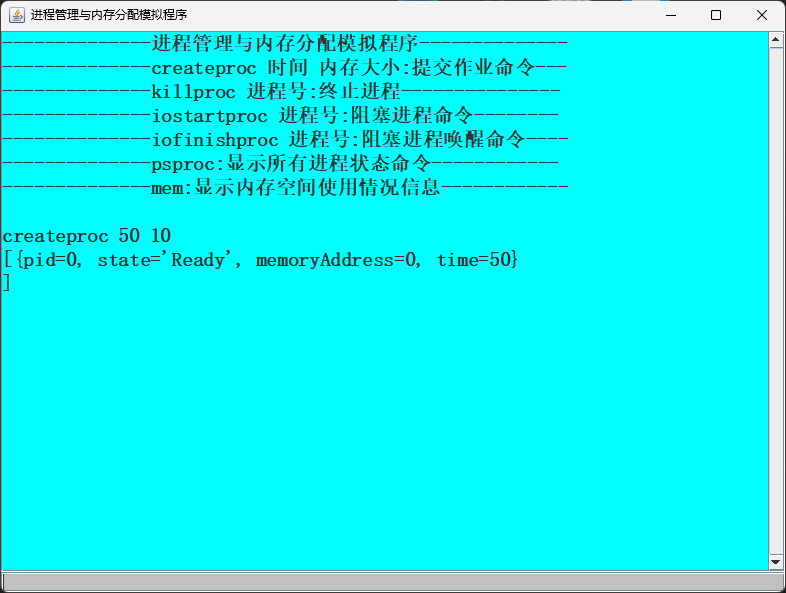
\includegraphics[width=0.5\textwidth]{img/2.png}
    \caption{创建进程}
\end{figure}

\newpage

\subsection{PCB、CPU满负荷运行}
\begin{figure}[htbp]
    \centering
    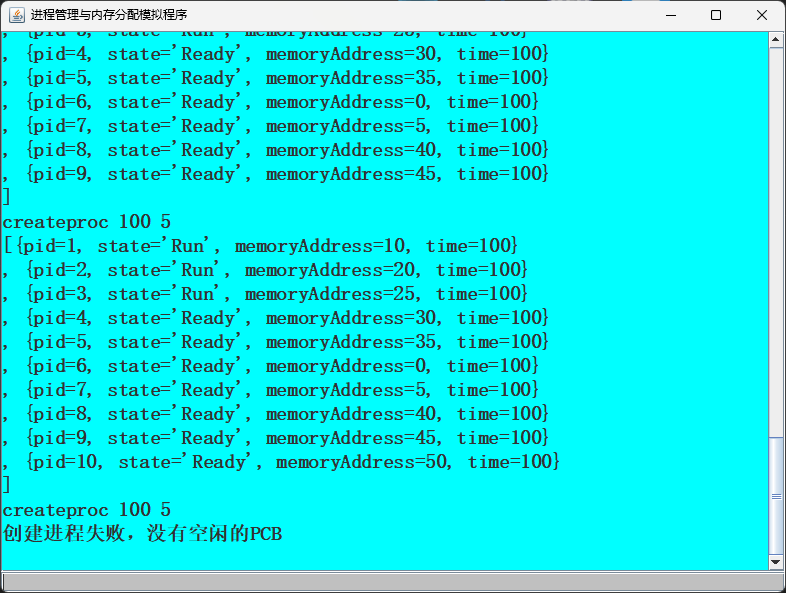
\includegraphics[width=0.55\textwidth]{img/3.png}
    \caption{PCB、CPU满负荷运行}
\end{figure}

\subsection{撤销进程}
\begin{figure}[htbp]
    \centering
    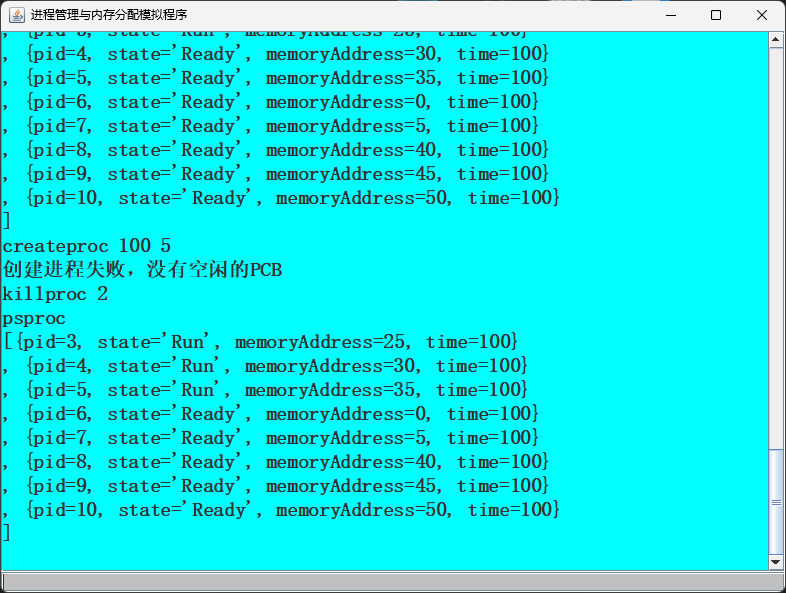
\includegraphics[width=0.55\textwidth]{img/4.png}
    \caption{撤销进程}
\end{figure}

\newpage

\subsection{阻塞进程}
\begin{figure}[htbp]
    \centering
    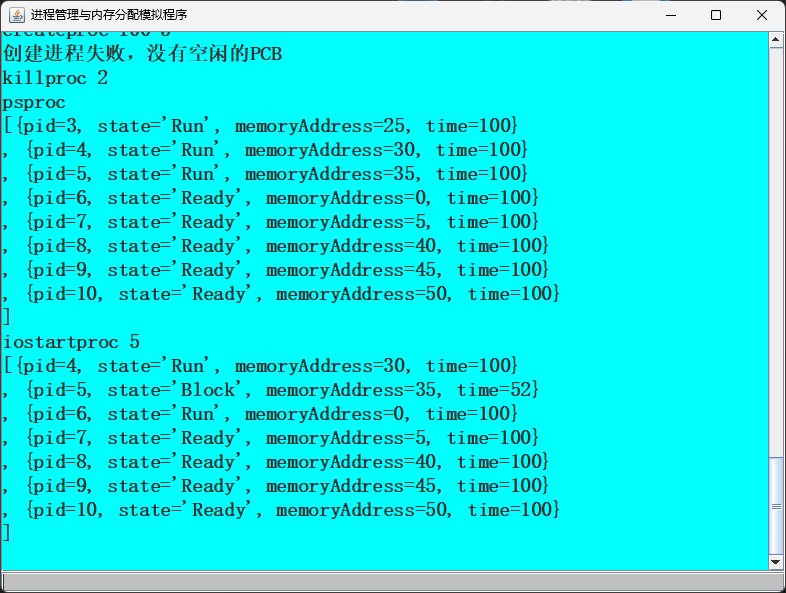
\includegraphics[width=0.55\textwidth]{img/5.png}
    \caption{阻塞进程}
\end{figure}

\subsection{唤醒进程}
\begin{figure}[htbp]
    \centering
    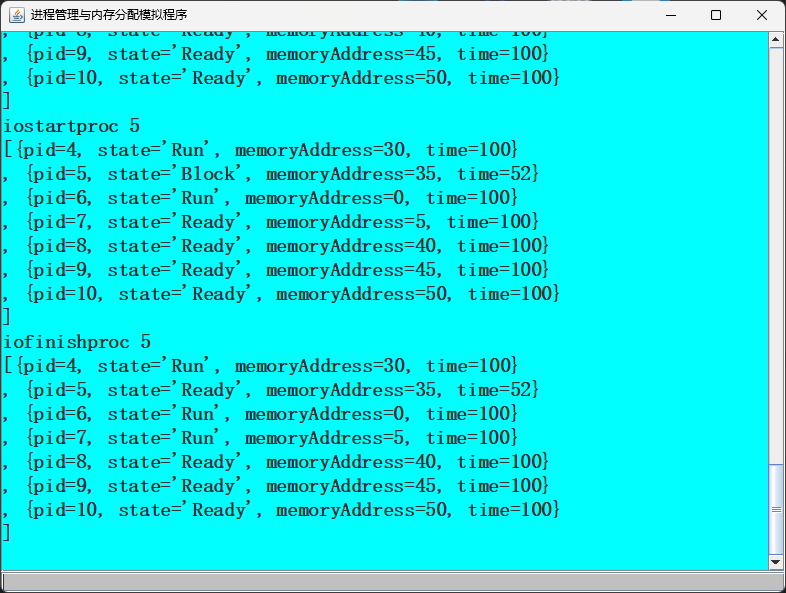
\includegraphics[width=0.55\textwidth]{img/6.png}
    \caption{唤醒进程}
\end{figure}

\newpage

\subsection{显示内存状态}
\begin{figure}[htbp]
    \centering
    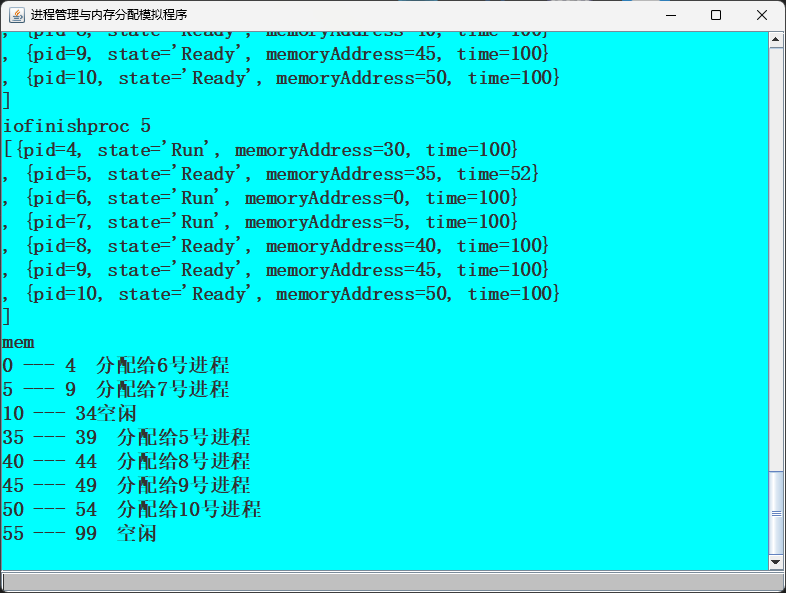
\includegraphics[width=0.55\textwidth]{img/7.png}
    \caption{显示内存状态}
\end{figure}


\section{总结与收获}
通过本次实验,我对进程管理和内存管理有了更深刻的理解。

在进程调度方面,本次实验使用了FCFS调度算法,即先来先服务调度算法,这种调度算法的优点是简单,容易实现,但是缺点是平均等待时间较长,不利于提高CPU的利用率,同时也不利于提高系统的吞吐量。实现起来比较简单,只需要将就绪队列中的第一个进程调度到运行队列中即可。逻辑清晰,代码简单。在实验的时候能够很好地复现出来,但是在实际的操作系统中,这种调度算法的使用场景并不多,由于本人水平有限,暂时还没有了解其他的调度算法的代码实现,希望在以后的学习中能够学习到其他的调度算法,提高自己的水平。

在内存管理方面,本次实验使用了可变分区的内存管理方式,即每个进程的内存大小不固定,根据进程的内存大小分配对应的内存块,这种内存管理方式的优点是能够充分利用内存空间,缺点是容易产生内存碎片,同时也不利于提高内存的利用率。实现起来比较简单,只需要将空闲内存块按照大小进行排序,然后遍历空闲内存块,找到第一个满足条件的空闲内存块即可。实际内存管理中,多采用段页式内存管理方式,这种内存管理方式能够很好地解决内存碎片的问题,同时也能够提高内存的利用率,但是实现起来比较复杂,需要考虑的条件很多,还需要继续学习,提高编程技巧

总的来说,本次实验收获很大,对进程管理和内存管理有了更深刻的理解,同时也提高了编程能力,希望在以后的学习中能够继续提高自己的水平,为以后的学习打下坚实的基础。

\section{附录}
\subsection{Properties包}
\subsubsection{FreeBlock.java}
\subsubsection{PCB.java}
\subsubsection{States.java}

\subsection{Service包}
\subsubsection{ManageMemory.java}
\subsubsection{ManagePCB.java}
\subsubsection{ManageProcess.java}
\subsubsection{Process.java}
\subsubsection{Schduler.java}

\subsection{View包}
\subsubsection{Console.java}
\end{document}